\def\year{2022}\relax
%File: formatting-instructions-latex-2022.tex
%release 2022.1
\documentclass[letterpaper]{article} % DO NOT CHANGE THIS
\usepackage{aaai22}  % DO NOT CHANGE THIS
\usepackage{times}  % DO NOT CHANGE THIS
\usepackage{helvet}  % DO NOT CHANGE THIS
\usepackage{courier}  % DO NOT CHANGE THIS
\usepackage[hyphens]{url}  % DO NOT CHANGE THIS
\usepackage{graphicx} % DO NOT CHANGE THIS
\urlstyle{rm} % DO NOT CHANGE THIS
\def\UrlFont{\rm}  % DO NOT CHANGE THIS
\usepackage{natbib}  % DO NOT CHANGE THIS AND DO NOT ADD ANY OPTIONS TO IT
\usepackage{caption} % DO NOT CHANGE THIS AND DO NOT ADD ANY OPTIONS TO IT
\DeclareCaptionStyle{ruled}{labelfont=normalfont,labelsep=colon,strut=off} % DO NOT CHANGE THIS
\frenchspacing  % DO NOT CHANGE THIS
\setlength{\pdfpagewidth}{8.5in}  % DO NOT CHANGE THIS
\setlength{\pdfpageheight}{11in}  % DO NOT CHANGE THIS
%
% These are recommended to typeset algorithms but not required. See the subsubsection on algorithms. Remove them if you don't have algorithms in your paper.
\usepackage{algorithm}
\usepackage{algpseudocode}
\usepackage{amssymb}
\usepackage{amsmath}

%
% These are are recommended to typeset listings but not required. See the subsubsection on listing. Remove this block if you don't have listings in your paper.
\usepackage{newfloat}
\usepackage{listings}
\lstset{%
	basicstyle={\footnotesize\ttfamily},% footnotesize acceptable for monospace
	numbers=left,numberstyle=\footnotesize,xleftmargin=2em,% show line numbers, remove this entire line if you don't want the numbers.
	aboveskip=0pt,belowskip=0pt,%
	showstringspaces=false,tabsize=2,breaklines=true}
\floatstyle{ruled}
\newfloat{listing}{tb}{lst}{}
\floatname{listing}{Listing}
%
%\nocopyright
%
% PDF Info Is REQUIRED.
% For /Title, write your title in Mixed Case.
% Don't use accents or commands. Retain the parentheses.
% For /Author, add all authors within the parentheses,
% separated by commas. No accents, special characters
% or commands are allowed.
% Keep the /TemplateVersion tag as is
\pdfinfo{
/Title (Towards a robot partner reducing ambiguities using perspective taking)
/Author (Anthony Favier, Shashank Shekhar, Rachid Alami)
/TemplateVersion (2022.1)
}

% DISALLOWED PACKAGES
% \usepackage{authblk} -- This package is specifically forbidden
% \usepackage{balance} -- This package is specifically forbidden
% \usepackage{color (if used in text)
% \usepackage{CJK} -- This package is specifically forbidden
% \usepackage{float} -- This package is specifically forbidden
% \usepackage{flushend} -- This package is specifically forbidden
% \usepackage{fontenc} -- This package is specifically forbidden
% \usepackage{fullpage} -- This package is specifically forbidden
% \usepackage{geometry} -- This package is specifically forbidden
% \usepackage{grffile} -- This package is specifically forbidden
% \usepackage{hyperref} -- This package is specifically forbidden
% \usepackage{navigator} -- This package is specifically forbidden
% (or any other package that embeds links such as navigator or hyperref)
% \indentfirst} -- This package is specifically forbidden
% \layout} -- This package is specifically forbidden
% \multicol} -- This package is specifically forbidden
% \nameref} -- This package is specifically forbidden
% \usepackage{savetrees} -- This package is specifically forbidden
% \usepackage{setspace} -- This package is specifically forbidden
% \usepackage{stfloats} -- This package is specifically forbidden
% \usepackage{tabu} -- This package is specifically forbidden
% \usepackage{titlesec} -- This package is specifically forbidden
% \usepackage{tocbibind} -- This package is specifically forbidden
% \usepackage{ulem} -- This package is specifically forbidden
% \usepackage{wrapfig} -- This package is specifically forbidden
% DISALLOWED COMMANDS
% \nocopyright -- Your paper will not be published if you use this command
% \addtolength -- This command may not be used
% \balance -- This command may not be used
% \baselinestretch -- Your paper will not be published if you use this command
% \clearpage -- No page breaks of any kind may be used for the final version of your paper
% \columnsep -- This command may not be used
% \newpage -- No page breaks of any kind may be used for the final version of your paper
% \pagebreak -- No page breaks of any kind may be used for the final version of your paperr
% \pagestyle -- This command may not be used
% \tiny -- This is not an acceptable font size.
% \vspace{- -- No negative value may be used in proximity of a caption, figure, table, section, subsection, subsubsection, or reference
% \vskip{- -- No negative value may be used to alter spacing above or below a caption, figure, table, section, subsection, subsubsection, or reference

\setcounter{secnumdepth}{0} %May be changed to 1 or 2 if section numbers are desired.

% The file aaai22.sty is the style file for AAAI Press
% proceedings, working notes, and technical reports.
%

% Title

% Your title must be in mixed case, not sentence case.
% That means all verbs (including short verbs like be, is, using,and go),
% nouns, adverbs, adjectives should be capitalized, including both words in hyphenated terms, while
% articles, conjunctions, and prepositions are lower case unless they
% directly follow a colon or long dash
\title
{
Human-Aware 
Planning with Communication: \\ While Keeping Itself in Human's Shoes a Robot Plans for Both 
%is in Human's Shoes   
% Towards a robot partner reducing\\ ambiguities using perspective taking
}
\author{
    %Authors
    % All authors must be in the same font size and format.
    Anthony Favier\textsuperscript{\rm 1,2},
    Shashank Shekhar\textsuperscript{\rm 1},
    Rachid Alami\textsuperscript{\rm 1,2}
}
\affiliations{
    %Afiliations
    \textsuperscript{\rm 1}LAAS-CNRS, Universite de Toulouse, CNRS, Toulouse, France\\
    \textsuperscript{\rm 2}{Artificial and Natural Intelligence Toulouse Institute (ANITI)}

    % email address must be in roman text type, not monospace or sans serif
    \{anthony.favier, sshekhar, rachid.alami\}@laas.fr
}

\begin{document}

%%%%% SYMBOLS DEFINITION %%%%%
\newcommand{\worldstates}{\mathcal{S}}
\newcommand{\worldstate}{s}
\newcommand{\fluent}[3]{\mathcal{F}^{#1#2}_{#3}}
\newcommand{\prop}{\varphi}
\newcommand{\allprops}{\Phi}
\newcommand{\predicate}{\mathcal{P}}
\newcommand{\predval}{v}
\newcommand{\agent}{\lambda}
\newcommand{\beliefs}{\mathcal{B}}
\newcommand{\human}{H}
\newcommand{\robot}{R}
\newcommand{\places}{\mathcal{P}}
\newcommand{\place}{p}
\newcommand{\unknown}{UnKw}
\newcommand{\known}{Kw}
\newcommand{\missedactions}{\mathcal{M}}
\newcommand{\loc}[1]{loc(#1)}
\newcommand{\obs}[1]{obs(#1)}
\newcommand{\dom}[1]{dom(#1)}
\newcommand{\observable}{\texttt{OBS}}
\newcommand{\inferrable}{\texttt{INF}}
%%%%%%%%%%%%%%%%%%%%%%%%%%%%%%

\maketitle

\begin{abstract}
We consider human-aware task planning for a team of a human and a robot sharing joint tasks with known task objectives.

\end{abstract}

\section{Introduction}
With the increasing penetration of sensor networks, advancements in robotic technology, the Internet of Things (IoT), etc., multi-robot systems are becoming ubiquitous, and the complexity of the tasks these (multiple) autonomous robots can handle is constantly increasing.
Robots collaborating and (or) interacting with humans, for example, a robot hands over a water bottle to a human, robots achieving joint goals or getting a common joint-task done with the help of humans available in the environment, a robot getting its task done while receiving some routine helps when needed from a human, etc., is seldom seen in our day to day life, will soon become ubiquitous, too.

Consider a scenario in which you (a \textit{human} agent) want to prepare, together with your robot, some pasta in your kitchen. This joint task comprises several components and activities in the real world, for example, pasta packets kept in the cupboard in the kitchen or a room, lidding a pot, turning on a furnace, salt, adding some salt to the pasta, etc. Sometimes the needed objects might be accessible only to you (the robot) from your (its) current position, while some are accessible to both. 
Like this subclass of collaborative tasks, its multiple instantiations across many other real-world domains exist, e.g., homes, offices, hospitals, etc.

In such scenarios, naturally the human agent would want to work alongside the robot but without being bothered too much and too often, or sometimes she is too lazy to perform an action assuming that the robot will do it instead, even if it takes longer to achieve the overall joint-task. The human agent may \textit{choose} to leave the place during the task execution. Although, in these cases, the human agent is considered a fully cooperative and rational partner, she cannot be managed like an artificial agent (a fully controllable agent). But, the robot can always influence her behavior. 
% by eliciting her actions and emulating her mental state
%Even 
That gives rise to one crucial aspect of human-robot collaboration: A robot should not only plan for their joint actions but also predict and emulate human decisions and actions (and sometimes human's reactions, as well) to seamlessly achieve the joint-task together. 
The robot must put itself in the shoes of the human agent, which helps sometimes \textit{prohibit} the human agent execute an action with a detrimental effect on the overall joint-task, e.g., the action ends up destroying a resource essential to achieving the joint-task. 
Moreover, it also helps the robot to create a situation that will \textit{promote} some actions of the human agent, which is ``relevant'' to achieving the joint-task.       
% In this setting, it is common to compute a policy for all agents using a central engine. This policy is executed by
% the agents in a decentralized manner, and agent communication
% is performed through explicit actions.


Considering these above scenarios: There has been a series of work on
human task modelling and human-aware task planning to build a task planner focusing on human-robot collaboration and (\textit{partially}) dealing with those important issues we discussed earlier~\cite{alami2006toward,montreuil2007planning,alili2009planning,lallement2014hatp,de2015hatp,lallement2018hatp}.

Recently, in~\cite{BuisanA21,buisan:hal-03684211}, unlike the previous approaches, the authors propose a more suitable framework for these sub-class of HRI problems, which is comprising a \textit{dual} HTNs (Hierarchical Task Networks~\cite{naubooks0014222}) joint-task specification model: One model is for the human agent, and the other is for the robot. 
They assume that a domain modeler with expertise (in robotics, human-human collaboration, and human psychology) is available to describe HTN specifications for such collaborative planning paradigms. The dual HTNs describe agents' capabilities, initial beliefs, shared tasks, world dynamics, common ground (or their understanding of the world), etc. While the modeler also describes some \textit{hypothetical} hidden variables that are implicit, to capture a human's mood, intentions, etc., and they are hard to observe. Both these models are with the robot, while it plans its actions based on these joint specification models, and predicts and emulates human actions, decisions, and reactions.    

HATP-EHDA~\cite{buisan:hal-03684211} is a dual HTNs based solver that is the state-of-the-art planner. In principle, it is able to model and handle most of the cases that may arise in human-robot collaboration during planning. Without loss of generality, it assumes that agents \textit{decide} to act (e.g., pushing a heavy box, moving, noop, idle, etc.) one after the other. 
It generates a policy tree comprising human and robot actions. Note that a human is an uncontrollable agent, so even if she is being rational and collaborative, it is hard to determine her ``next'' action upfront -- describes the impact of those hidden variables.
Therefore, for a sound execution, after every robot action, the policy tree gets branched on all possible \textit{choices} available for the human.

HATP-EHDA assumes that if the robot executes an action, the human's belief gets updated, along with the robot's belief, or vice versa. It means that all the action execution is observable to both these agents. It is a \textit{major} drawback of the solver, since it is not always the case in reality. For example, in the pasta preparation scenario, suppose the human leaves the kitchen, and before she arrives back in the kitchen, the robot \textit{adds} some salt to the pasta, \textit{lids} the pot, and \textit{turns} on the furnace. 
Later, when the human arrives in the kitchen: What would be the new belief of the human? Certainly, she will observe that the furnace is {\sc on}, and also the pot is closed. But what about ``there is already some salt in pasta?'' Which creates divergence in the agents' belief states. 
% In such scenarios, 
To simplify the reasoning process over multiple task models, we assume that the robot is always aware of the ground truth. That means that we ignore the uncertainty associated with what the human does when the robot is absent. 
And any advancement in this direction is left for future work. 


% can handle different initial distinct beliefs
In this work, we address the issue of execution time observability, and propose a principled approach to handle such belief divergences during the planning phase. 
We address it via explicitly modeling and planning with communication actions. 
To do so, we extend the existing HATP-EHDA framework. We thank the modeler again for explicitly specifying, which state variables/fluents are \textit{observable} (an persistent effect of an action, e.g., turning on the furnace, which the human can observe with the help of \textit{situation assessment} (SA)~\cite{cite?} -- SA helps the human to assess the environment), \textit{inferrable} -- an effect of an action being executed by some other agent, which can only be inferred when the agent sees the action being performed by the other agent, e.g., robot adding some salt to the pasta and human sees it doing so. 
The latter can be informed about the exact value of the inferrable state variables, otherwise, to manage the belief alignment.   
%- both human and robot beliefs will be updated 

Communication paradigms like text, visual, speech, etc., are prerequisites for building a communication protocol among multiple agents. However, effective use of the modality is essential to achieve the motivation behind their development, say, a seamless agent collaboration. Moreover, using communication among the agents, too much and too little, can hamper or delay the overall task achievement. So, deciding on ``How to communicate?'' is crucial, but it is equally significant to decide ``If, When, and What to Communicate?'' 
We assume that a natural language-based speech modality is available, while our proposed algorithm optimally decides if, when, and what to communicate via planning with communication actions.
%

The paper is structured as follows: We first build a relevant background to understand this framework and discuss the related work. We then discuss the methodology: which includes modeling and planning with communication actions. 
After that, we present the results and show examples where handling the belief divergences is effective and how HATP-EHDA is ineffective under those scenarios. We compare the overall effectiveness of our approach and prove that it does not use communication more than needed (avoids verbosity) in the process. We conclude with a summary, discussion, and future work.

\section{Background and Related Work}

**********************

**********************


% what is known ? our understanding of the world
General context, towards robot partner. 

% what is unknown ? the gap we want to fill
% how and why ? your rational and purpose/hypothesis 

\textbf{Choice to reduce ambiguities [example, as introduction]}:
Let's assume the human and the robot have to cook together and at some point salt needs to be added to a dish. The robot adds salt to the dish while the human is away. When coming back, the human has no way to know if there is salt just by looking at the dish.
Then three cases can occur : 1) The human considers that the robot didn't add salt, thus they will to add more, 2) The human considers that the robot added salt, so the goal is reached, 3) the human prefers to directly ask the robot if it added salt. 
Humans are rational, so they will rarely blindly act without at least asking the state of the shared plan. However, whatever case we are in, an ambiguity will remain for the human, and we are able to predict it. Thus, we decide to proactively reduce the ambiguity by communicating about their belief divergences or the missed actions. This communication might seem optional in some situations but having a plan without ambiguities in the context of a shared goal is often much better than a plan with fewer steps but where agent aren't sure about what they have to do.

\clearpage
\section{Related Work}

\begin{itemize}
    \item Some refs from ICRA paper ? (Devin theory of mind) 
    \item Human activity model, hierarchical HTN
    \item HATP general
    \item HATPEHDA (ICRA)
    \item explicit communication, multi agent 
    \item belief divergences, non verbal com
\end{itemize}

\section{Background}
HATPEHDA concept and definitions

The work \cite{buisan:hal-03684211} already support collaborative task planning while maintaining distinct beliefs/knowledge for each agent. This work is itself an extension of HATP \cite{hatp?} having one search thread for a shared plan resulting in two coordinated plan streams. The last work HATPEHDA proposes a two threads search. Based on this work, we enhanced the task planner with a few concept linked to perspective taking and observability in order to reduce the ambiguities that may happen in a collaborative task. First we predict the situation assessment of an agent. On the other hand, we look for belief divergences that have a detrimental influence on the plan in order to fix them with communication. We also check observability of action execution to update beliefs with different types of effects.

Agents can have a shared goal but no shared plan. There is no plan negotiation between the agents, so the robot is only able to estimate what the human will do and plan its own actions according to that.

\subsection{HATPEHDA background/basis and definitions}

The main structure manipulated by our planner is the \textbf{agent}, more precisely two will be represented, the \textit{human} and the \textit{robot}. Each agent has their own \textbf{beliefs}, \textbf{action model}, \textbf{agenda}, \textbf{plan} and \textbf{triggers}. The planner has to use their action models and beliefs to decompose the tasks in their agenda into primitive tasks (actions) that are inserted in their plan. By doing so, it also has to update the beliefs of each agent and to model their reaction by executing the triggers. \cite{buisan:hal-03684211}.

The agents, robot and human, have each a distinct action model modeled with HTNs. The robot HTN starts with the goal given to the robot and describes how to decompose that abstract goal into several actions. The human HTN represents the anticipation by the robot of the human plan and possible actions in a given situation. Other formalism like POMDP or PDDL could be used to describe the agents' action models as soon as they provide the next possible actions of an agent in a given state. Especially the human one which is an estimation.

The planner has a goal creation mechanism, especially for the human, based on goal-directed or situation-directed task creation.

The planning algorithm is implemented as a search involving two threads: 1) the robot task-based plan search using the robot action model 2) the estimation of the human task-based plan search using the human action model.

While HTN-R corresponds to the controllable part  (from the robot point of view) of the (shared) plan, HTN-H represents the contingent part of the plan: the decisions and actions of the human. 

Hence, the obtained plan has two streams (one for the human and one of the robot) and is conditional. Alternatives correspond to human decision: choosing to act or not, making one (out of several choices).

As a result, HATP/EHDA allows to clearly separate what is planned for the robot and what the human can potentially do with respect to the task at hand. Besides, it allows to also:
\begin{itemize}
    \item deal with cases where the task is only given to the robot and not shared by the human
    \item manage the creation of a shared goal
    \item provide a mean to implement elicitation, by the robot, of decisions or reactions of the human
\end{itemize}
In our case the plan process starts:
\begin{itemize}
   \item with a goal given only to the robot: a task placed at the root of HTN-R (ex: Human asks the robot to achieve a goal)
   \item or with a shared goal: the same task is placed at the roots of  the two HTNs (ex: Human says to the robot: "Let us do X")
\end{itemize}

Situation-directed task creation in HTN-H allows to model (potential) reaction by the human to a situation created by after a given action of the robot. This can be used in the planner to elicit a reactiion of the human.

\textbf{HTN formalism [in background ?]}:
An HTN \textit{planning problem} is the 3-tuple $\langle d, S_0, \mathcal{D} \rangle$, where $d$ is the sequence of (primitive or abstract) tasks to solve, $S_0$ is an initial state as in classical planning, and $\mathcal{D}$ is an HTN \textit{planning domain}. Specifically, an HTN \textit{planning domain} is the pair $\mathcal{D}=\langle\mathcal{A},\mathcal{M}\rangle$ where $\mathcal{A}$-the primitives of the domain-is a finite set of operators as before, and $\mathcal{M}$ is a finite set of \textit{methods}. A \textit{method} is a tuple consisting of the name of the method, the abstract task that the method is used to solve, a precondition specifying when the method is applicable (like an operator's precondition), and a \textit{body} indicating which tasks are used to solve the task associated with the method. The method-body is a sequence of primitive and/or abstract tasks. 

The planning process works by selecting applicable reduction methods from $\mathcal{M}$ and applying them to abstract tasks in $d$ in a depth-first manner. In each iteration this will typically result in $d$ becoming a "more primitive" sequence of tasks. The process continues until $d$ has only primitive tasks left. At any stage in the planning process, if no applicable method can be found for an abstract task, the planner essentially "backtracks" and tries an alternative method for an abstract task refine earlier.

\textbf{Computing next possible agent actions / refining agenda [nothing new here, in hatpehda background ?]}:
% The refinement of the HTNs is mostly done thanks to the function $refineAgenda()$. This function keeps refining the agenda of an agent in a given state until reaching a not done primitive task at the first spot. It returns a refinement which is list of decomposition, one for each applicable methods. Each decomposition is a list of the obtained subtasks which starts with a not done primitive task. The second parameter the function $refineAgenda$ can be used to specify with which beliefs the refinement has to be done. 
The action model of each agent is described with a HTN. Thus, the process to compute (or estimate in the human case) the next possible actions of an agent is very close to classic HTN refinement.
The classic planning process for HTN planning problem consist in selecting applicable reduction methods from $\mathcal{M}$ and applying them to abstract tasks in $d$ in a depth-first manner. In our contribution the planning process slightly differs from the classic process since the goal is to compute or estimate all possible next actions in a given state. 
Here, $d$ corresponds to what we call the agenda of the agent. To compute the next possible actions the agent's agenda is refined. To do so the first task in the agenda is popped, and all applicable reduction methods are applied to the task resulting is search branches with different subtasks. The process is repeated for each created branch until reaching a primitive task in each of them. The primitive tasks from each search branch constitute the set of all possible next actions of the agent.
A search branch can refine into nothing but if all search branches refine into nothing then the first task popped from the agenda is done, so the next task in the agent's agenda is popped and refined. 
A search branch, corresponding to a list of subtasks, is called a decomposition. The list of all obtained decompositions is called a refinement.  


\section{Materials and Methods}
% what did you do ?



\subsection{Knowledge representation and observability definitions}

Our formalism is close to the SAS+ Formalism applied to HTN.(Probably to remove, might bring more confusions than explanations)

\textbf{Word state}: 
Let $\worldstates$ be the set of all possible world states. World states are defined by a same set of fluents. Each world state is fully described by the value of all its fluents at a given time i.e. $\forall\worldstate\in\worldstates, \worldstate=\{ \fluent{\worldstate}{}{} \}$.

\textbf{Fluent}: 
A fluent $\fluent{\worldstate}{}{}$ is a multi-valued state variable associated to a finite domain $\dom{\fluent{\worldstate}{}{}}$ partially describing the state of the world at a given time.

% (introduce loc ?)
% The observability type of fluents is qualified through the relation $\obs{ \fluent{\worldstate}{}{} } \in \{ \observable, \inferable \}$. 

e.g. Considering the following fluent $\fluent{\worldstate}{}{temp\_water}$, if initially the water is hot then $\fluent{\worldstate_0}{}{temp\_water}=hot$.

\textbf{Belief divergence}: 
We note $\fluent{\worldstate}{,\agent}{}$ a fluent evaluated in the perspective of an agent $\agent$. Thus, for a given real state of the world $\worldstate\in\worldstates$, the robot and the human can have different values for the same fluent. We call such mismatch a belief divergence.

e.g. $(\fluent{\worldstate_0}{,\robot}{temp\_water}{}=hot) \neq (\fluent{\worldstate_0}{,\human}{temp\_water}=cold)$

\textbf{Two distinct Beliefs}: 
We call beliefs of an agent $\agent$, noted $\beliefs_\agent$, the belief state in which this agent thinks the world is in, i.e. the set of all fluents evaluated in their perspective at a given time: $\beliefs_\agent=\{ \fluent{\worldstate}{,\agent}{} \}$. It is important to note that we use two distinct belief states during the planning process. On one hand, we consider the beliefs of the robot $\beliefs_\robot$ which are obtained through perception and effects of robot actions and decisions. And as we consider the planner as being part of the robot, we assume that $\beliefs_\robot$ is the ground truth estimation for the planner. On the other hand, we consider the human's belief state $\beliefs_\human$ which is only estimated by the robot by doing some perspective-taking reasoning during the planning process (and before ?).

\subsection{Place-based observability model}

We introduce a place-based model of observability. An agent observes and can only observe what happens in their current place, this includes action executions and fluent values.

\textbf{Places}: 
A place is an area defined a priori in the environment. Let $\places=\{ \place_i \}$ be the set of all defined places. Agents are always situated in a place or moving between them. Two agents situated in the same place are said to be co-present. Actions are always performed in a place. (Most?) State variables are associated to a place.

\textbf{Observation of an action execution}: 
The execution of an action performed by an agent $\agent$ is observed by all agents that were co-present with $\agent$ either before or after the action. The co-presence is checked both before and after to cover navigation actions.

\textbf{Observability of fluents}:
Each (most?) fluent is associated to a place $\place \in \places$ through the relation $\loc{ \fluent{\worldstate}{}{} }=\place$. These relations help to describe the world state by expressing where the fluents are effective and observable. (If $\loc{ \fluent{\worldstate}{}{} } = \varnothing $ then the fluent is ubiquitous). These relations can be dynamic for example when the fluent describes a property linked to a moving entity. Currently, the location of a fluent has to be updated manually in the domain if it is dynamic (we should go for an "entity-based" description of the world state to automatically update).

The observability type of each fluent is constant and defined initially through the relation $\obs{ \fluent{\worldstate}{}{} } \in \{ \observable, \inferable \}$. 
The first value $\observable$ means that the fluent is observable. A fluent is observed by an agent only if it is observable and if that agent is in the place associated to the fluent. 
Note that places can be symbolic and not only physical/geometric to represent more complex situation. For instance, let's consider the fluent $\fluent{\worldstate}{}{at\_o}$ describing the position of an object \textit{o}. The object is in the kitchen inside a cupboard that can either be open or closed. This situation can be modeled as follows :
\begin{itemize}
    \item $\fluent{\worldstate}{}{at\_o}=cupboard$
    \item $\obs{ \fluent{\worldstate}{}{at\_o} }=\observable$
    \item $\loc{ \fluent{\worldstate}{}{at\_o} } \in \{ kitchen, closed \}$
\end{itemize}
The relation $\loc{ \fluent{\worldstate}{}{at\_o} } = kitchen$ corresponds to when the cupboard is open, which means any agent in the place $kitchen$ can observe the object. On the other hand, when the cupboard is closed, $\loc{ \fluent{\worldstate}{}{at\_o} } = closed$, the agent cannot observe the object.

The other value $\inferable$ qualifies inferable fluents. A fluent is inferable if its value isn't observable but can be inferred by attending an action affecting that fluent. For instance, by observing someone adding salt to a dish we infer that there is now salt in the dish, although the salt in the dish isn't observable. It means that without attending the action execution it's impossible to tell if there salt just by looking at it. Thus, when an action affects inferable fluents only the co-present agents gets their beliefs updated. We later refer to actions affecting inferable fluents as actions with inferable effects (resp. with observable effects).


\subsection{Beliefs updates}

Agents' beliefs are updated by four different processes: 1) performing an action, 2) attending inferable effects, 3) assessing the situation, and 4) communicating about a relevant belief divergence.  

\textbf{Performing actions / Inferable effects}: 
When an agent performs an action its own beliefs are always directly updated with the action's effects.

The other agent's beliefs are updated about these effects through two mechanisms. The first one, that will handle observable effects, is the situation assessment and is detailed just after. 
The second one concerns inferable effects. As mentioned before, only agents that observed the action execution get their beliefs updated with the inferable effects.

For now, we assume that if we estimate that the human will perform a task not observable by the robot then it should remain quite simple like a series of deterministic actions. Basically, we currently do not handle more complex cases where the human has multiple choices of actions while not being observable. Considering this hypothesis, the robot beliefs are always updated with the effects of human actions, weither they are co-present or not.

\textbf{Situation Assessment}:
The idea is to predict the situation assessment of an agent and update their beliefs according to what they can see in their current place. When executed, each agent $\agent$ updates their beliefs with the ground truth value of every observed fluents, i.e. for every observable fluents ($\obs{ \fluent{\worldstate}{}{} } = \observable$) located in their place ($\loc{\fluent{\worldstate}{}{}} = \fluent{\worldstate}{}{at\_\agent}$), we have $\fluent{\worldstate}{,\agent}{} \gets \fluent{\worldstate}{}{}$. The situation assessment is executed after every action execution. This way, the agent's beliefs are updated either with the observable effects of an action performed by another co-present agent, or with the observable effects they missed when entering another place. 
Note that since the ground truth is actually the robot beliefs, this situation assessment is only effective for other agents, so here the human. 

\textbf{Relevant belief divergences checking}:
We want to detect if a belief divergence influences the plan of the human, i.e. if when using the human beliefs containing belief divergences induces different human actions than the ones expected using the ground truth beliefs. If so, the belief divergences are qualified as relevant. Indeed, a belief divergence can wrongly affect the applicability of a human action, its cost and its effects. 
Any difference in the human plan makes it either not applicable in reality, more expensive or with undesired effects. There are some rare cases of belief divergences inducing a different plan still applicable, with a similar cost and no undesired effects. But for now we omit those cases, and we consider relevant belief divergences as always detrimental. 
Note that there can be belief divergences not affecting the plan which will not be considered as detrimental.

To check if there are some relevant belief divergences we proceed as follows. When refining the human agenda to estimate their next possible actions, we first use the human beliefs $\beliefs_H$. The process is repeated but considering the robot beliefs $\beliefs_R$ (ground truth). The two obtained refinements are then compared to check if they are the same. Two refinements are considered to be the same if they respectively have the same decompositions, i.e. if, in both refinements, each decomposition respectively has the same type, subtasks and if their actions have the same applicability, cost and effects. 
If a difference is spotted we consider that there are relevant belief divergences to align, but we don't know which ones yet.

\textbf{Identify the relevant divergences and communicate}: 
Once the presence of relevant belief divergences has been confirmed they have to be identified. All divergences between $\mathcal{B}_R$ and $\mathcal{B}_H$ are first computed. Then the divergence's corrections are simulated one after another (i.e. $ \fluent{\worldstate}{,\human}{i} \gets \fluent{\worldstate}{,\robot}{i}$) and the human agenda is refined again in order to compare the new refinement with the one previously obtained with $\beliefs_\robot$. We keep simulating combination of divergence corrections in a breadth-first (search) manner until the refinements are the same, which means that all the relevant divergences have been identified. In the worst case, the two refinement are not the same until reaching the last combination which corresponds to all divergences being corrected, thus where $\beliefs_\human$ and $\beliefs_\robot$ are the same. So the obtained refinements will necessarily be the same which guarantees the ending of our algorithm. After having identified the divergences to correct in order to obtain the same refinements, the corresponding communication action is inserted in the robot's plan to inform the human about their relevant belief divergences and to correct them.
    
Communication actions are supposed to be instantaneous and able to correct several divergences at once. For now they are inserted right before the detected erroneous human action. (A more complex reasoning could be added to identify the optimal place to insert the communication action in the plan). 

% \textbf{Choice to reduce ambiguities}:
% In the case of a shared goal, let's assume that the human didn't observe the robot performing an action with only inferable effects, so when coming back the human has no way to tell if the action has been done just by looking at the scene. 
% Then three cases can occur : 1) The human considers that the robot didn't perform the action, thus the human will try to perform it again, 2) The human considers that the robot performed the action, so the plan execution continues, 3) the human prefers to directly ask the robot if it performed the action. 
% Humans are rational, so they will rarely blindly act without at least asking the state of the shared plan. However, whatever case we are in an ambiguity will remain for the human, and we are able to predict it. Thus, we decide to proactively reduce the ambiguity by communicating about their belief divergences or the missed actions. This communication might seem optional in some situations but having a plan without ambiguities in the context of a shared goal is often much better than a plan with fewer steps but where agent aren't sure about what they have to do. Communication help to compel the human actions.


\subsection{Algorithm (Optional maybe ...)}
MAYBE OPTINAL because it involves mechanisms not introduced (or maybe we should introduce them in the background ?) like the triggers and the WAIT/IDLE actions.

The refinement of the HTNs is mostly done thanks to the function $refineAgenda()$. This function keeps refining the agenda of an agent in a given state until reaching a not done primitive task at the first spot. It returns a refinement which is list of decomposition, one for each applicable methods. Each decomposition is a list of the obtained subtasks which starts with a not done primitive task. The second parameter the function $refineAgenda$ can be used to specify with which beliefs the refinement has to be done. 

The returned refinement in Alg.~\ref{alg:ap_ref_all} contains the subtasks obtained through the refinement of the agenda after a potential belief alignment, application of the actions, situation assessment and triggers.

\begin{algorithm}
\caption{Get applied refinement ALL}\label{alg:ap_ref_all}
\begin{algorithmic}
\Require $h\_name$: human name, $r\_name$: robot name, $ags$: all agents

\State $ref \gets refAgenda(ags, ag\_name)$

\State $ref\_r \gets refAgenda(ags, r\_name)$ \Comment{H only}
\If{$relevantDivergences(ref, ref\_r)$} \Comment{H only}
    \State $alignBeliefsWithComAction()$
    \State $ref \gets refAgenda(aligned\_ags, h\_name)$
\EndIf

\For{$decomp$ in $refinement$}

    \State $result \gets applyOperator(dec, ag\_name)$ 
    \If{$notApplicable(result)$}
        \State \texttt{add wait, idle or end}
    \Else
        \State $applyOperator(dec, r\_name)$ \Comment{H only}
        \State $applyInferableEff(dec, h\_name)$ \Comment{R only}
        \State $humanSituationAssessment()$
        \State $checkTriggers()$
        \State $updateDecomp(decomp)$
    \EndIf
\EndFor

\State \Return ref

\end{algorithmic}
\end{algorithm}



\section{Results}
% what results did you get ?

Present example : Probably cooking example turning fire (situation assessment) and adding salt (relevant divergence). Show plan without our contribution. Then show what we obtain with our contribution.

Think about other configuration of the same scenario for other cases ? Here prevent action with undesired effects. Should find also applicability and cost.

Explicitly say that previous version of hatpehda do not handle belief divergences at planning level, it could if specification is given in the domain. That's why fails here but were able to handle them in specific scenario (example previous paper/thesis).

Quantitative: We can randomize or use all combination of initial state : pasta location, starting agent, initial agent location, (initial belief divergence ?). Make statistics on applicability of plans with and without contribution 

Qualitative :

Domain description:

\begin{itemize}
    \item $\places = \{ kitchen, room \}$
    
    \item $\fluent{\worldstate}{}{salt\_added}$
        \subitem $\dom{\fluent{}{}{}} = \{ true, false \}$
        \subitem $\loc{\fluent{}{}{}} = kitchen$
        \subitem $\obs{\fluent{}{}{}} = \inferable$

    \item $\fluent{\worldstate}{}{pot\_fire}$
        \subitem $\dom{\fluent{}{}{}} = \{ on, off \}$ 
        \subitem $\loc{\fluent{}{}{}} = kitchen$ 
        \subitem $\obs{\fluent{}{}{}} = \observable$ 
    
    \item $\fluent{\worldstate}{}{at\_\{\robot,\human\}}$
        \subitem $\dom{\fluent{}{}{}} = \places$ 
        \subitem $\loc{\fluent{}{}{}} \in  \places$ 
        \subitem $\obs{\fluent{}{}{}} = \observable$ 

    \item $\fluent{\worldstate}{}{at\_\{pasta\}}$
        \subitem $\dom{\fluent{}{}{}} = \places \cup \{ \robot, \human \}$ (when holding)
        \subitem $\loc{\fluent{}{}{}} \in  \places$ 
        \subitem $\obs{\fluent{}{}{}} = \observable$ 
    
\end{itemize}

\begin{figure}
    \centering
    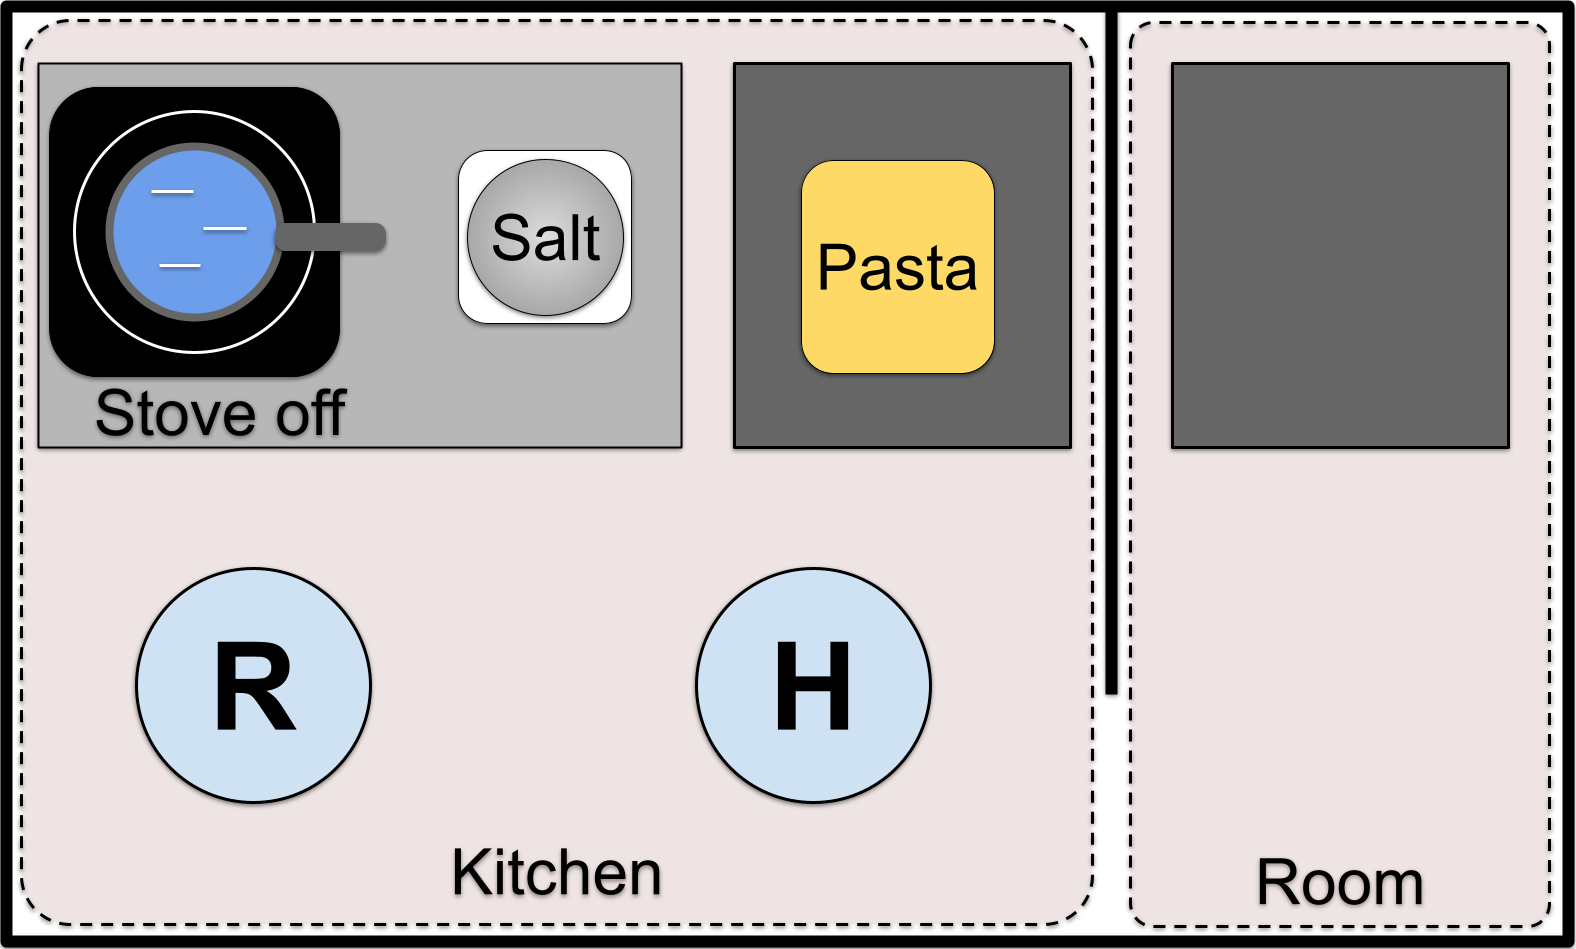
\includegraphics[width=0.8\linewidth]{figures/scene.png}
    \caption{Scene cooking}
    \label{fig:scene}
\end{figure}

Task description in HTN depicted in Fig.~\ref{fig:htn}

\begin{figure}
    \centering
    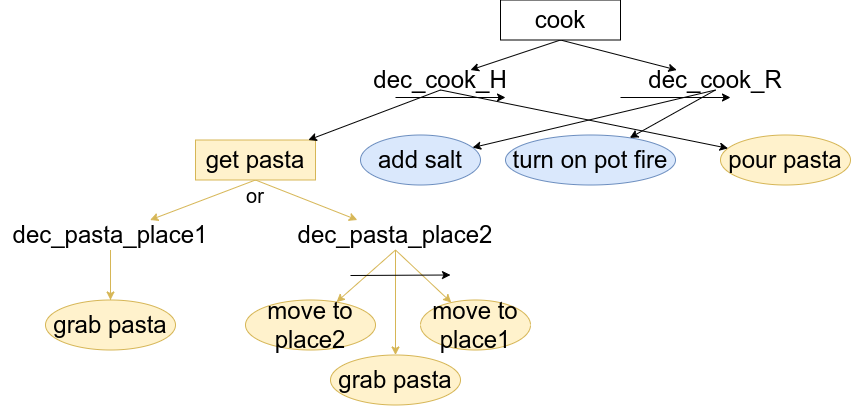
\includegraphics[width=\linewidth]{figures/htn.png}
    \caption{HTN, cook task description. Done conditions are added to primitive tasks to lighten the htn description. This can be modeled with dedicated methods with classical HTN model.}
    \label{fig:htn}
\end{figure}

\begin{figure*}
    \centering
    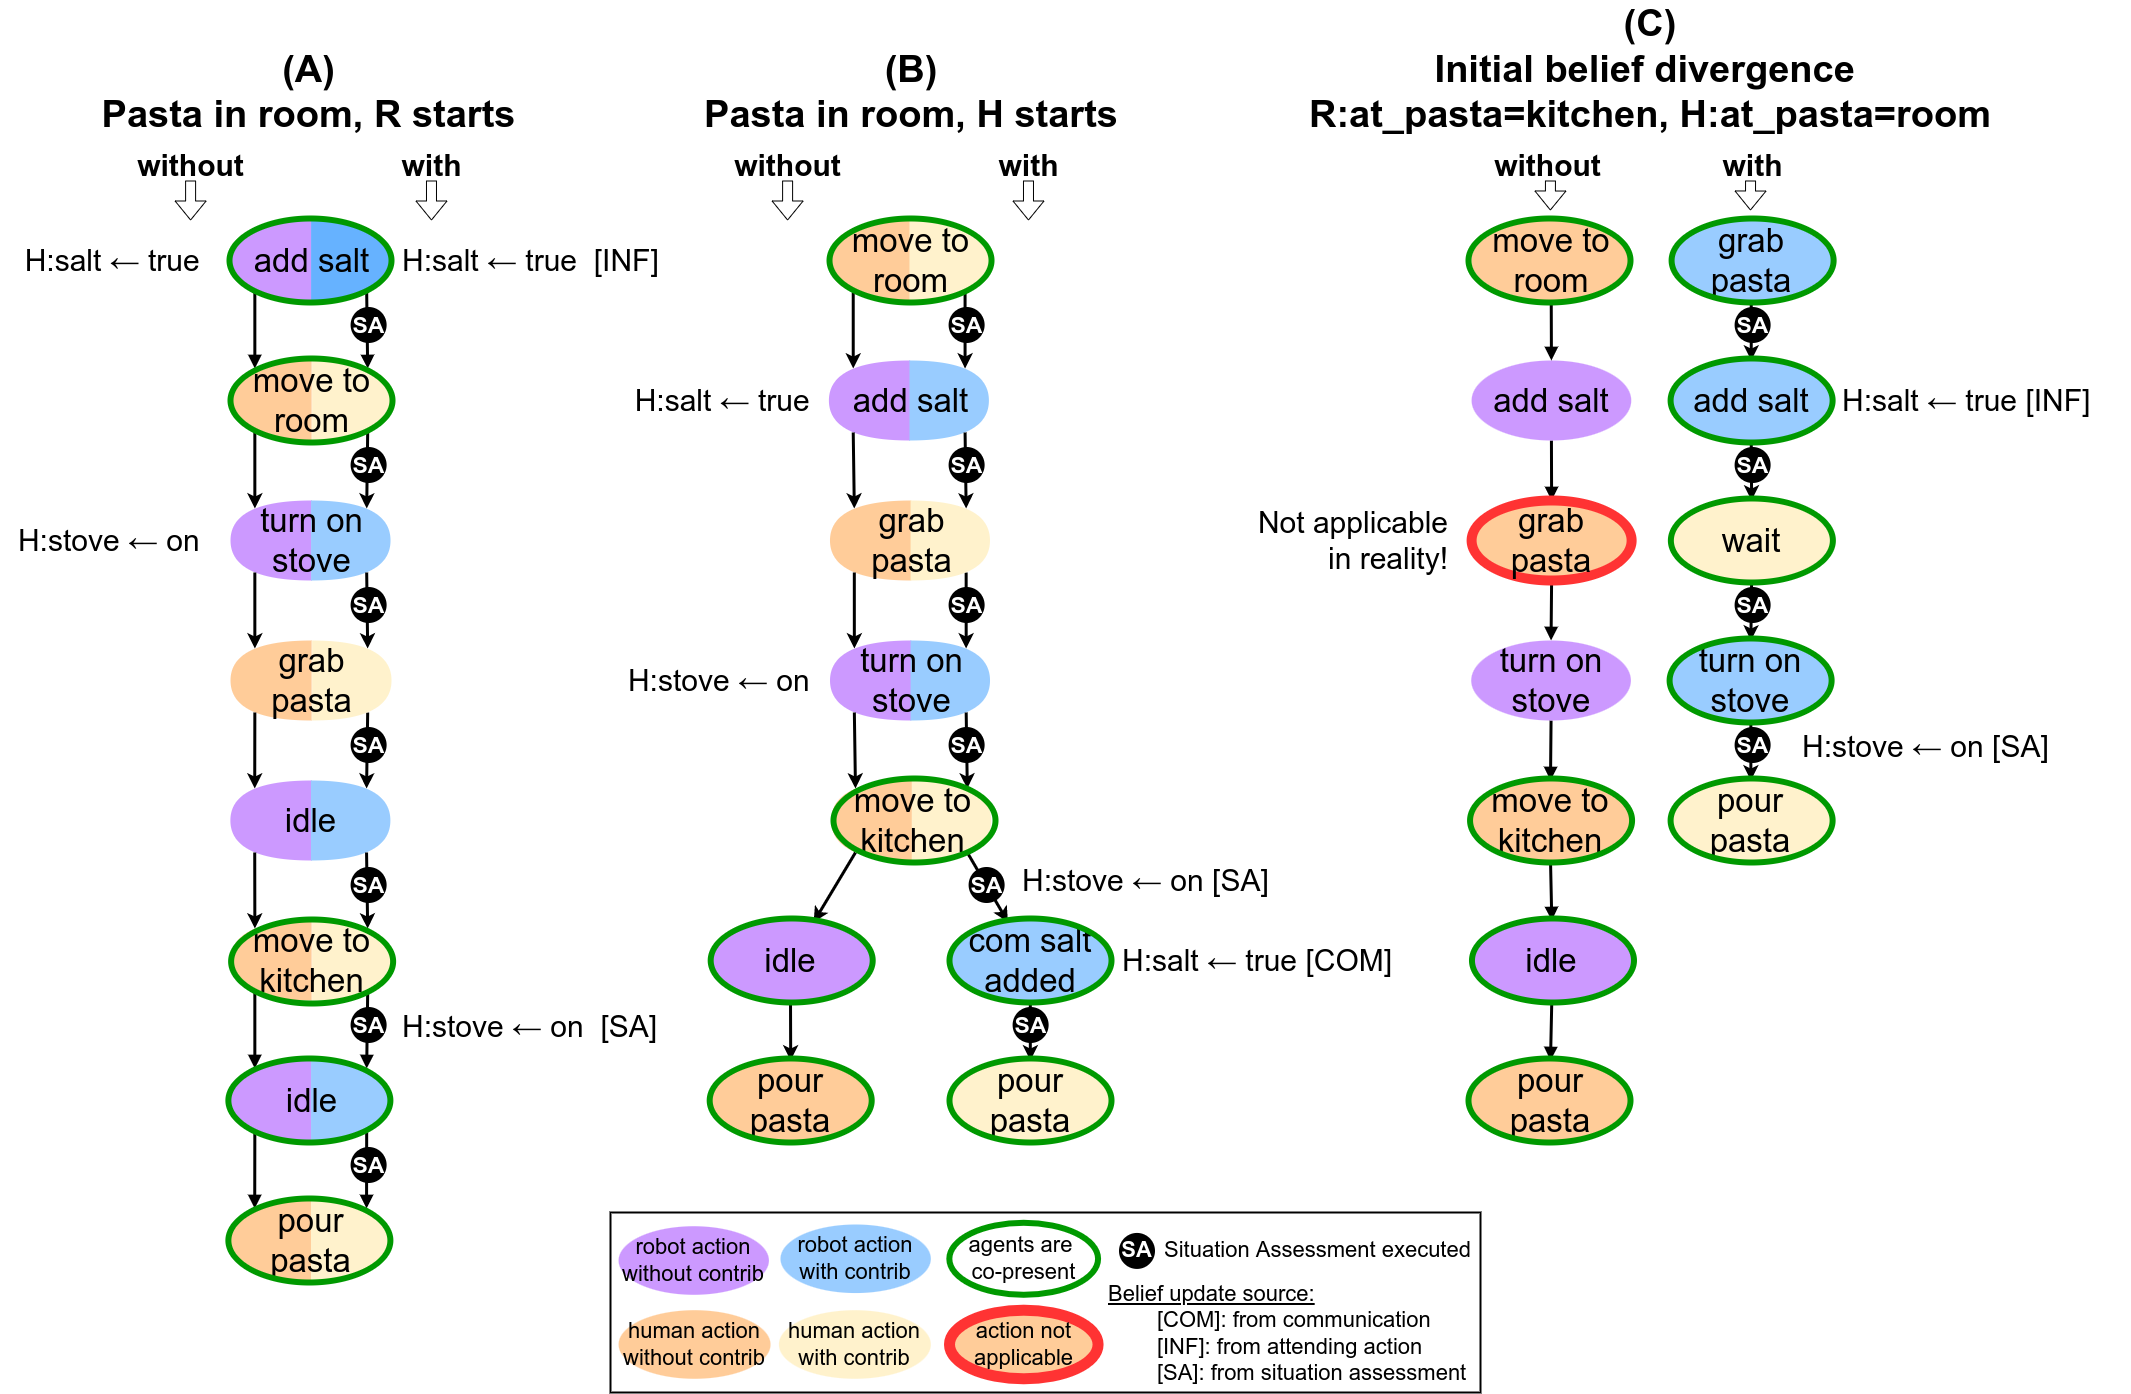
\includegraphics[width=\linewidth]{figures/example_cook.png}
    \caption{Caption}
    \label{fig:scenarios}
\end{figure*}


Scenarios:
\begin{itemize}
    \item \textbf{pasta in same place (0-1)}
        \subitem normal execution
    
    \item \textbf{pasta in another place, R starts (72)}
        \subitem w/o: Agents are omniscient, H knows instantly about the effects of R actions even without observing the actions
        \subitem w/: H sees salt action and assess the fire on action when coming back. Thus, no com required, same plan than w/o, but beliefs have been updated differently
        
    \item \textbf{pasta in another place, H starts (73)}
        \subitem w/o: Agents omniscient again, H knows about all R actions instantly
        \subitem w/: R predicts H will miss both actions but will be able to assess the pot fire action execution when back in place1 but can't be sure about salt action. Decides to com to remove ambiguity
    
    \item \textbf{initial belief divergence on pasta location(R:place1 H:place2) (8-9). The robot brought the pasta closer before the human comes}
        \subitem w/o: Plan isn't actually applicable with ground truth knowledge (grab pasta, no pasta here)
        \subitem w/: Relevant belief divergence detected. R com to correct the relevant divergence and make H plan applicable
    
\end{itemize}

\section{Discussion}
% how do the results fill the gap ?

Point out ambiguities (created both by the lack of situation assessment and belief alignment) in the plans without contribution. Then, explain how we removed them. 

\section{Conclusion}
% what does this mean for us going forward ?

FUTURE WORK:
\begin{itemize}
    \item A more elaborated formula for observability than co-presence. Using geometrical reasoning with a physic simulator.
    \item Use an entity-based world description to be able to automatically update the $\loc{\fluent{\worldstate}{}{}{}}$.
    \item A more complex reasoning to decide where to insert the communication action in the plan.
\end{itemize}

\bibliography{bib.bib}

\end{document}
